\section{Communication network}

The communication network is crucial for \projectname{} to work.
When designing a communication network that have to scale it is important to choose the right structure.
There are different ways when designing such a network but identical for them all is they need to support the structure of M, S and B as seen in section~\ref{sec:application_structure}.

One of these solutions is to make a structure where M, S and B talk to each other with a level of security. 
The security aspect would be implemented with a form of session key. 
This key would be used to determine if a session between a B and a S is valid.
Another solution is to provide no security aspect and let it be up to the users and / or company to keep drones safe from intruders.
This would lessen the communication between the users and the servers.  
It would also decrease the load on Master and Slave's database. 
On the down side the system could be considered not safe because it would be possible to tamper with the drones.
As this is a system where it is important that the integrity is high, evidence is not tampered with, and where the outcome of an unauthorized user controller a drone could be devastating, it is important to deliver some form of security.

\begin{figure}[!h]
    \centering 
    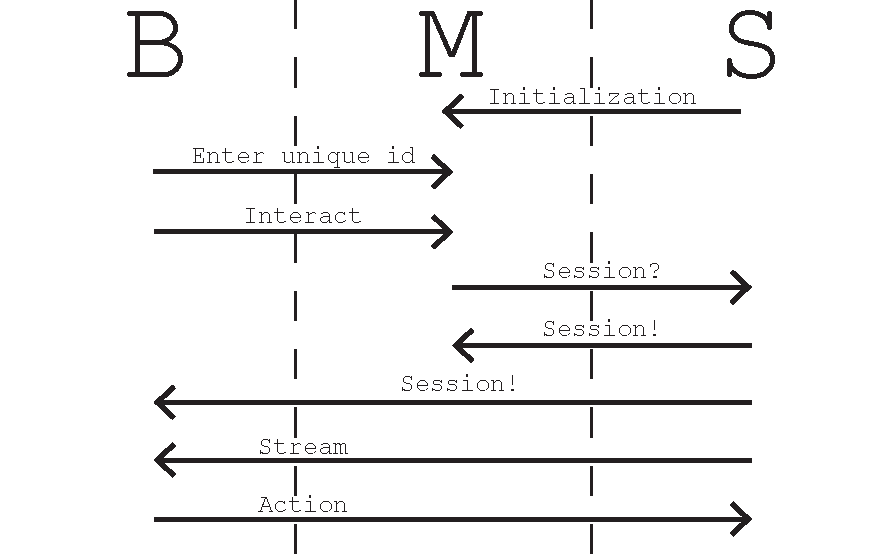
\includegraphics[width=\textwidth]{gfx/activity_diagram.pdf}
    \caption{Activity diagram of the communication network between B, M, and S}
    \label{fig:activity_diagram}
\end{figure}

This lead to a solution where sessions is designed to keep the integrity and secure evidence as seen in figure~\ref{fig:activity_diagram}. 
As seen in the figure there is designed a level of security because of the sessions. It is not possible for a B to interact with a drone without having a session with a drones S.

When a drone is purchased a Slave is setup at the location where the drone is going to operate.
The Slave sends an initializing message to Master, informing Master that a new drone has entered the system.
Master adds the drone with the IP and location of the Slave, along with the drone's unique identifier.
If Master receives an initializing message from a Slave with a drone identifier that is already in the system, it will destroy any session that correlates with that drone. The sessions is destroyed because if one or more sessions are granted and S sends its initializing message it is safe to assume that S either disconnected or crashed and all sessions keys are invalid.
Furthermore if the IP of Slave differs from that of the drone it will be updated.
If a user tries to interact with a drone the system behaves differently. A session key will be made on Slave, this key will be send to Master and giving to the user. With this session key it is possible for the user to communicate directly with the Slave without the Master.

\begin{figure}[!h]
    \centering 
    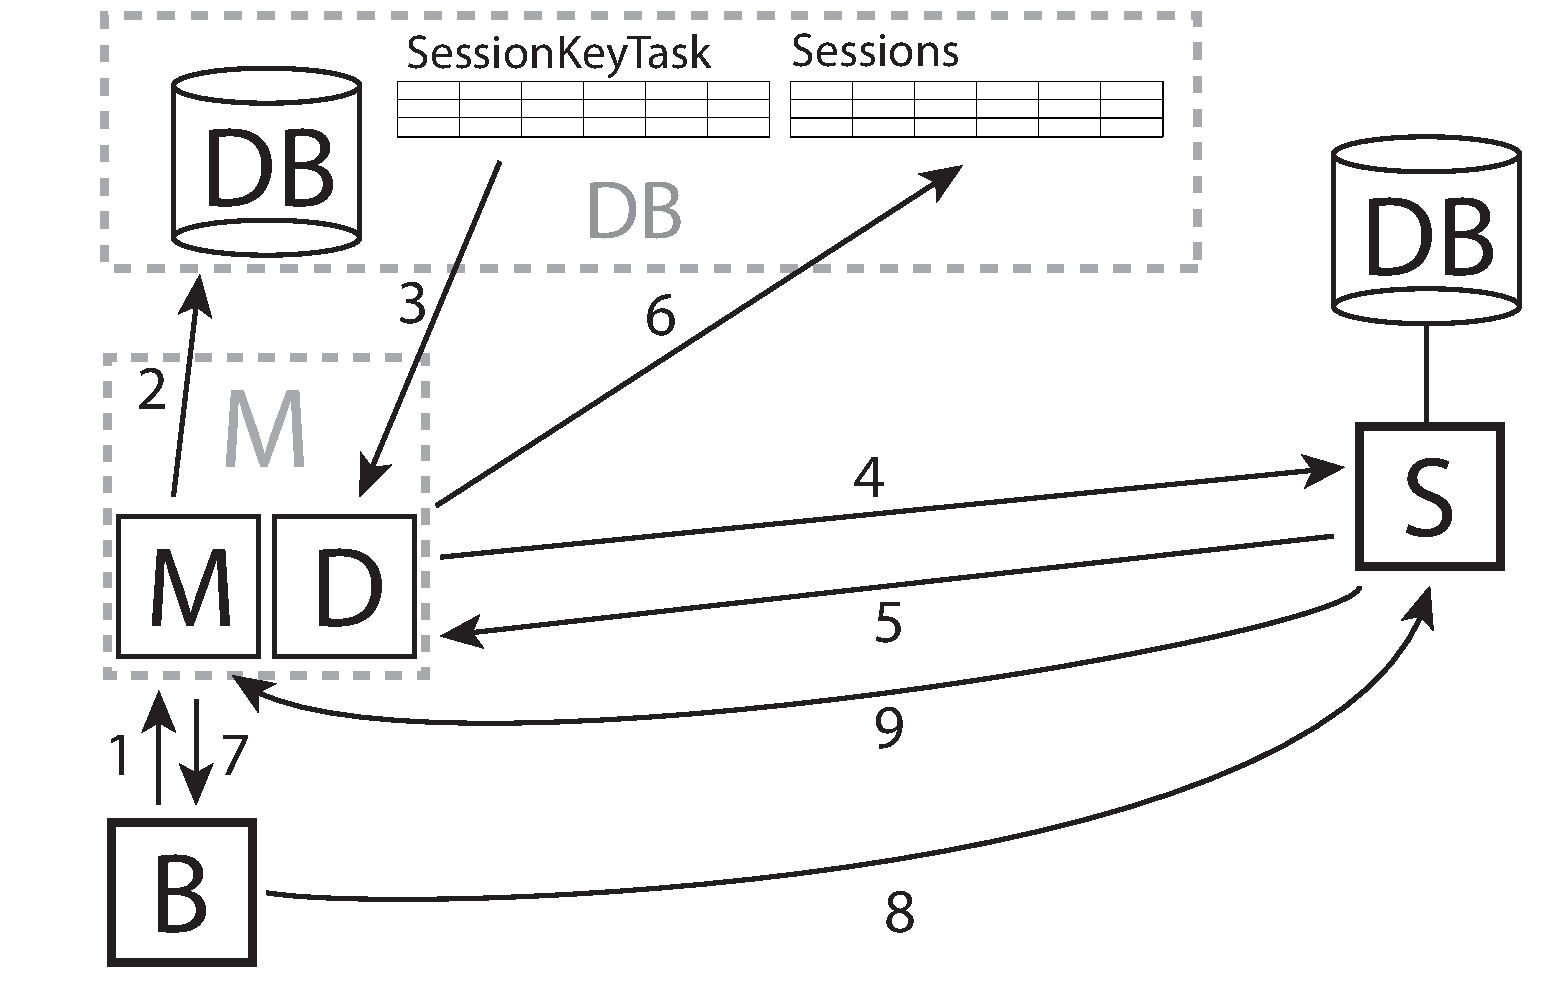
\includegraphics[width=\textwidth]{gfx/sessionkey_communication.pdf}
    \caption{Session key communication between B, M, and S}
    \label{fig:sessionkey_communication}
\end{figure}

This behavior can be seen in figure~\ref{fig:sessionkey_communication}. 

Session keys have been designed for security reasons.
Firstly they were designed to ensure that only one user at a time could control a drone.
Secondly it ensured that unauthorized users do not have the possibility of controlling a drone.

\begin{enumerate}
	\item Request send from B to M about getting a session key to interact with a drone.
	\item M inserts this request in its database table called SessionKeyTask.
	\item D scans the database table SessionKeyTask, when it sees a new entry it select it and then deletes it from the table.
	\item D requests a session key from S parred with the drone the user wants to interact with.
	\item S makes a random generated string with uppercase, lowercase letters and number. This string is used as the session key. S updates its database with this session key and then sends it back to D on M.
	\item D inserts the newly received session key into the session table of M.
	\item M then contacts B with the session key.
	\item B uses this session key to access S and through it interact with the drone.
	\item A Timeout happens if B and S does not communicate for 10 seconds.
\end{enumerate}

Communication between the actors in the system are crucial. 
Therefore it was important to make a method or methods for communicating between them. 
One method could be to make a service which handles all these requests on each server. 
The problem however is that with only one service they are a possibility for introduction a bottleneck to the system.
Another solution is to make a service for each communication level. One service that handles sessions, a service that handles control commands, and a service that handles initial messages from Slaves see section~\ref{sec:application_structure}.

This lead to a solution where the different actors in the system delivered and / or depended on services'.

The interface of the communication network can be seen in figure~\ref{fig:communication_network}.

The communication network of \projectname{} uses four different ports for providing its services:

\begin{itemize}
	\item Port A - service port for sending and receiving drone control commands.
	\item Port B - service port for receiving and sending initial messages.
	\item Port C - service port for sending and receiving session information including session keys.
	\item Port Web - service port for sending and receiving web specific information.
\end{itemize}

\begin{figure}[!h]
    \centering 
    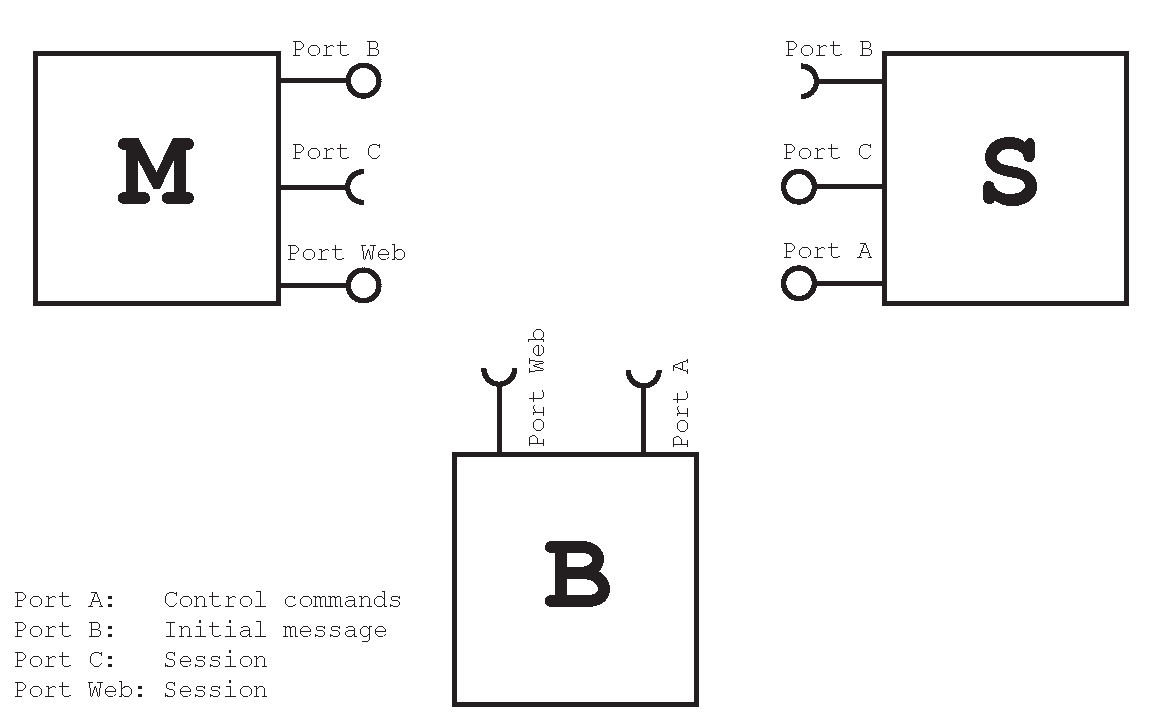
\includegraphics[width=\textwidth]{gfx/communication_network.pdf}
    \caption{Communication network between B, M, and S}
    \label{fig:communication_network}
\end{figure}

